\documentclass{article}
\usepackage{tikz}
\usepackage{graphicx}
%\usepackage{pgfplots}
%\usepgfplotslibrary{polar}

\begin{document}
\thispagestyle{empty}
\begin{figure}
\centering
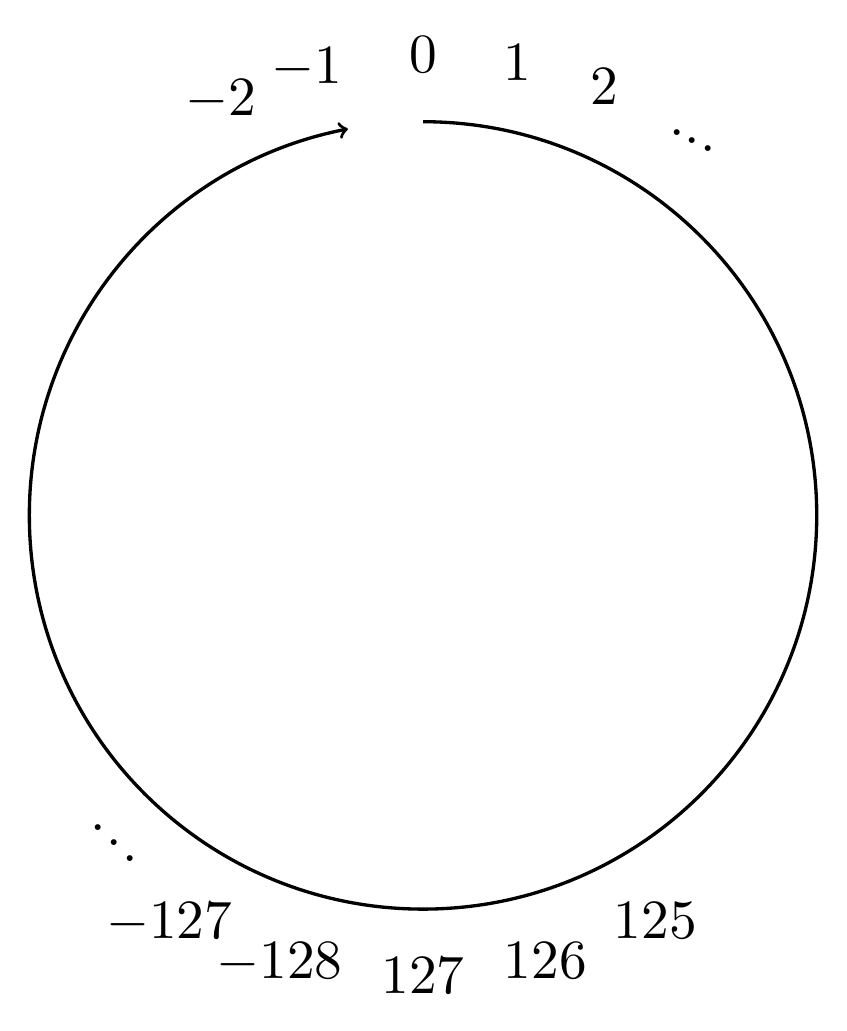
\begin{tikzpicture}
	%\draw[->] (0,0) circle (5cm);  % -> doesn't work
	\draw[very thick,->] (0,5) arc (90:-259:5cm);

	% annotate the int
	%\draw (0,5) node[anchor=south] {$\Large 0$};  % 0 too small
	%\draw (0,5.5) node[anchor=south] {\scalebox{2}{$\Large 0$}};  % cf. https://tex.stackexchange.com/questions/3703/make-equations-large
	\node[above]       at (0, 5.5) {\scalebox{2}{$\Large 0$}};
	\node[above right] at (0.9, 5.4) {\scalebox{2}{$\Large 1$}};
	\node[above right] at (2, 5.1) {\scalebox{2}{$\Large 2$}};
	\node[above right] at (3, 4.7) {\scalebox{2}{.}};
	\node[above right] at (3.2, 4.6) {\scalebox{2}{.}};
	%\node[above right] at (3.35, 4.45) {\scalebox{2}{.}};
	\node[above right] at (3.4, 4.5) {\scalebox{2}{.}};

	\node[above left] at (-0.9, 5.3) {\scalebox{2}{$\Large -1$}};
	\node[above left] at (-2, 4.9) {\scalebox{2}{$\Large -2$}};
	%\begin{polaraxis}
	%	\draw (4.8,10) -- (5.2,10);
	%\end{polaraxis}

	\node[below]       at (0, -5.5) {\scalebox{2}{$\Large 127$}};
	\node[below right] at (0.9, -5.3) {\scalebox{2}{$\Large 126$}};
	\node[below right] at (2.3, -4.8) {\scalebox{2}{$\Large 125$}};
	\node[below left] at (-0.9, -5.3) {\scalebox{2}{$\Large -128$}};
	\node[below left] at (-2.3, -4.8) {\scalebox{2}{$\Large -127$}};
	\node[below left] at (-3.5, -4.2) {\scalebox{2}{.}};
	\node[below left] at (-3.7, -4.0) {\scalebox{2}{.}};
	\node[below left] at (-3.9, -3.8) {\scalebox{2}{.}};



\end{tikzpicture}
	\vspace{1cm}
	\caption{\huge In C, the addition of any two \texttt{signed int} (here for example $8\,$-bit) is nothing more than a compound clockwise rotation along the circle}
\end{figure}
\end{document}
